\documentclass[a4paper]{article}

\usepackage[dvipsnames]{xcolor}
\usepackage[T1]{fontenc}
\usepackage[utf8]{inputenc}
\usepackage{lmodern}

\usepackage[english]{babel}
\usepackage{csquotes}

\usepackage{graphicx}
\graphicspath{ {./images/} }

\usepackage[margin=0.6in]{geometry}

\usepackage[notes,backend=biber]{biblatex-chicago}
\bibliography{sample}

\begin{document}
\title{Unsupervised Learning - CS 4641}
\author{Omar Shaikh}
\maketitle

\begin{abstract}
    In this report, I cover two fundamental unsupervised machine learning algorithms: K-means and Gaussian Mixture Models. To do this, I select two different data-sets -- images of histopathologic-cancer tumors and the classic Iris Flower Dataset. First, I introduce each data-set and our unsupervised classification problem; then, I run the clustering algorithms on the datasets and describe my results, both before and after running the aforementioned dimensionality reduction algorithms. 
    
    The next section is neural network analysis on a single dataset. First, I rerun my neural network learner on two cases on only the dimension reduced dataset, and . In the comparative analysis section, I test each algorithm on the withheld testing data, showcasing the strengths and weaknesses of each while answering some questions.
\end{abstract}

\section{Neural Network Assessment \& Computer Specifications}
Before I begin, here is a general procedure I used for assessing each algorithm. If any change was made to the procedure, it is addressed in a following subsection.

\begin{enumerate}
  \item First, I withheld 10\% of the data-set, after shuffling, for final testing; the remaining 90\% fell into testing. I saved the random state to reproduce the splits.
  \item I split the training data into k-folds for cross validation, where k=10. If k is not defined, assume k=10
  \item Then, I used the mean of the classification accuracy on each k-fold (from the training data) as a baseline, picking hyper-parameters that improved this baseline.
  \item Finally, I would test on the dataset on the withheld 10\% 
\end{enumerate}
The computer used to train and test has an i7-7700HQ (clock speeds @ 3.8 GHZ), 32 GB of RAM, and an Nvidia GTX 1070 with 8 GB of VRAM. Whenever it was possible, I used all CPU cores (n\_jobs=-1 in sci-kit). Runtimes of algorithms should be considered in context of these specifications.

\textcolor{red}{Please note that the final evaluations of each dataset on the withheld testing data will occur in the comparative analysis section; the algorithm sections contain information regarding training and cross validation evaluation only!}

\section{Dataset \& Classification Problems}
\subsection{PCam Dataset \& Classification}

The first dataset I used (same as assignment \#1) is the CAMELYON dataset, collected by Department of Pathology of the Radboud University Medical Center (Radboudumc) in Nijmegen, The Netherlands \autocite{doi:10.1093/gigascience/giy065}. I found this dataset after searching for labelled cancer images datasets; because I wanted to explore machine learning on a computer vision classification problem, and the dataset size was quite large, it seemed like a good choice. 

Luckily, a Kaggle user edited a version of CAMELYON; images were converted to a .tif format, an accompanying CSV file labeled each image in the dataset, and duplicates were removed. The dataset has binary labels: either the cells have metastasized (1 label), or they have not (0 label). For the sake of speed, I chose to undersample this dataset such that N=X, instead of N=220025. The original and undersampled dataset will both have a 60-40 split. See figure 1 for a breakdown of the undersampled dataset. 

Finally, why this dataset? My family has an unfortunate genetic history with cancer, so a related project was generally of interest. Also, computer vision is considered a strength of deep neural networks -- working with an image based dataset would help me see if and why this is so.

\subsubsection{General Feature Engineering}
Although images provided were a 96x96 slide, only the center 32x32 contained tumor tissue. For classifiers used in this report, I cropped the images beforehand -- the outer region was merely provided to enable fully-convolutional models that do not use zero-padding\autocite{Kaggle-PCam}. For my CNN, I cropped the image regardless. I also normalized the pixel values to have zero mean, even though image pixel values have relatively homogeneous distributions. 

\begin{figure}
  \centering
  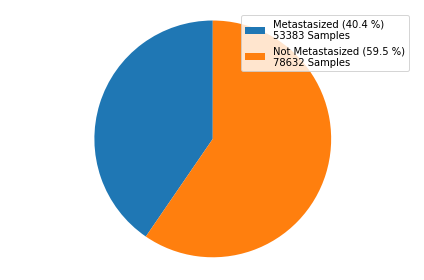
\includegraphics[width=0.4\textwidth]{images/pcamDistr.png}
  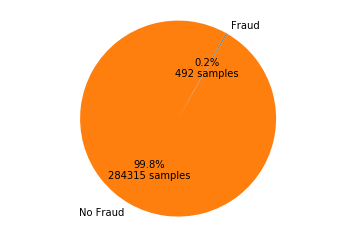
\includegraphics[width=0.4\textwidth]{images/fraudImg.png}
  \caption{Breakdown of the datasets; PCam (left), Credit Card Fraud (right)}
\end{figure}

\subsection{Credit Card Fraud Dataset \& Classification}

I found this dataset on Kaggle after searching for risk analytics challenges; it was collected during the a research collaboration between Worldline and the Machine Learning Group of ULB (Université Libre de Bruxelles) \autocite{dal2015calibrating}. This dataset poses a unique to me because it's highly imbalanced -- there are only a few (proportionally) samples of fradulent credit cards. Also, the actual credit card data (28 features, aside from the date and amount) were anonymized with PCA analysis; working with a dataset without having access to the original information itself was a unique challenge

A short except from the Kaggle challenge, along with figure 1, highlights the breakdown of the dataset:

\begin{quote}
The datasets contains transactions made by credit cards in September 2013 by European cardholders. This dataset presents transactions that occurred in two days, where we have 492 frauds out of 284,807 transactions [also a binary classification task]. The dataset is highly unbalanced, the positive class (frauds) account for 0.172 \% of all transactions \autocite{Kaggle-CreditCard}.
\end{quote}

Finally, why this dataset? I will be interning at Square this summer, potentially on the applied ML team, so working on this dataset would let me analyze data similar to what I would receive during my internship. Plus, who can say no to busting bad guys.

\subsubsection{Feature Engineering and Modified Model Assessment}
Before worrying about oversampling, I normalized the the date and amount values to lie within the same range as the PCA anonymized credit card data. Then, to deal with over-representation of one of the classes (transaction detected as a fraud), I needed to find a method to represent and evaluate the features in my dataset. Training the model would require us to under-sample the dataset, such that X and Y would have equal proportions of fraudulent and non-fraudulent datsets. 

The dataset was initially split into an original\_X\_test and original\_Y\_test -- this is a 90-10 split. Then, I generated an under-sampled dataset from all the 492 fraud instances. On this secondary under-sampled dataset, I split again with 80-20, creating a training and testing dataset. This is training set I ran cross validation on in the algorithm subsections. Finally, in the comparative analysis, I evaluated the under-sampled 20\% alongside the entire with-held 10\% with the ROC-AUC score.

Note that for the testing of this dataset, I would test two separate sets in comparative analysis: the entire dataset, and the withheld 20\% from the under-sampled subset. Because of severe overrepresentation problems, I will use the Area Under the Receiver Operating Characteristic Curve (ROC AUC) for the comparative analysis testing, instead of accuracy during model training.

\section{Decision Trees}
\subsection{PCam}

\subsection{Note on Feature Engineering}
Because of memory constraints I ran into with decision trees, I also had to choose between excluding color channels or a down-sampling to 16x16. A quick analysis showed that including color had empirically higher results (without pre-pruning or depth-limiting the tree). Different coloring between metastasized tissue and non-metastasized tissue may have lead to a key branch in the decision tree. 

\begin{center}
\begin{tabular}{ |c|c|c|c| } 
\hline
Feature Engineering Type & \begin{math}\mu\end{math} 10-fold score \\
\hline
Not including color & .58 \\ 
Including color \& downsampling & .65 \\ 

\hline
\end{tabular}
\end{center}
\subsubsection{Finding hyper-parameters}
For this dataset, I started with a grid search. Each run of K-Fold (k=10) took, on average, 1 minute, so 10 folds took about 10 minutes; however, trees with larger depth limits and more leaf nodes more time to train and test. Combined with nearly 100 different combinations of depth limits and pre-pruning leaf choices, finding an optimum hyper-parameter took an entire day. Figure 2 shows mean k-fold scores with respect to independent variables in the grid search, omitting larger depth limits, since model performance was decreasing. The following sets defined the search space: $leafLimit = depthLimit = \{ 10,  20,  30,  40,  50,  75,  100,  200,  500,  1000,  None \}$ and $ criterion = { entropy }$. The entropy function in criterion set is the same function described in lecture that was used to quantify information gain.

\begin{figure}
  \centering
  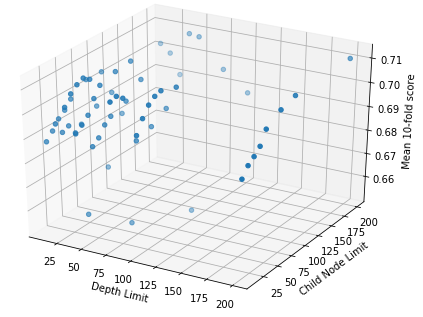
\includegraphics[width=0.4\textwidth]{images/gridSearch.png}
  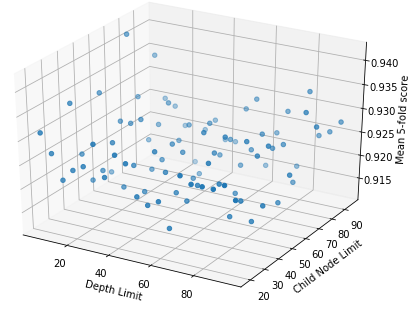
\includegraphics[width=0.4\textwidth]{images/gridSearchCredit.png}
  \caption{Hyper-parameter Grid Search with Decision Trees for PCam (left), Credit Card (right)}
\end{figure}

What's more than mildly disappointing is that the 10-fold accuracy when pruning leafs and limiting depth is only about 5\% better: 71\% compared to 65\%. When 50\% is random guessing, an accuracy rate of 71\% (where $leafLimit = depthLimit = 200$) is statistically significant -- but it's not impressive.
\subsection{Credit Card Fraud}
\subsubsection{Finding Hyper-parameters}
\begin{figure}
  \centering
  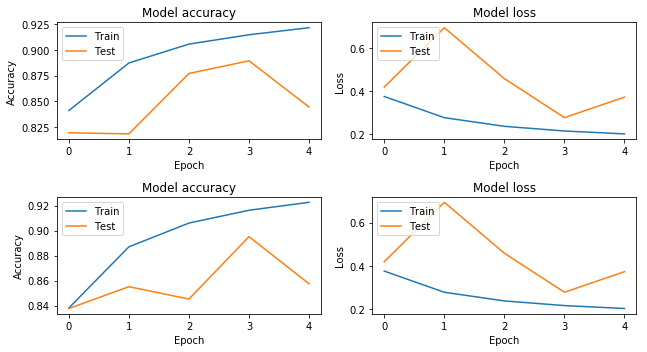
\includegraphics[width=1\textwidth]{images/nnplotcam.png}
  \caption{Complexity Curves with Batch-Norm before ReLU (top 2), after (bottom 2). Accuracy is $\mu$ 4-fold score.}
  {Note: Loss function is binary-cross entropy.}
\end{figure}
To find hyper-parameters, I played only with the undersampled dataset described in the dataset section. I discovered Sci-kit Learn's $gridSearchCV$ feature, and used the following choices for hyper-parameters: $leafLimit = depthLimit = list(range(2,100))$ along with $criterion = \{ gini,  entropy \}$. $gridSearchCV$ yielded the following results: $leafLimit = 76,$ $depth = 5,$ $criterion = entropy$ and a surprisingly high accuracy rate of 93.15\%. Hyper-parameter search in the specified search spaces took only 3.2 minutes; something I expected, since the dataset size and the number of features are smaller.
\section{Neural Networks}
\subsection{PCam}
For PCam, let k=4 for cross validation: this is because I don't have more GPU oomph. Each run of K-fold with 5 epochs took about 25 minutes; because I varied two combinations of neural network architectures, total training time took 3.33 hours.
\subsubsection{Finding Hyper-parameters}
I found that using batch-gradient descent in general greatly sped convergence of the loss function (binary-cross entropy), so training on less epochs (the other hyperparameter) was possible. One of the hyperparameters I also wanted to tweak was the positioning of the batch-normalization layer. Empirically, batch-norm should perform better after ReLU\autocite{Chollet-Comment}, although its positioning still remains a topic of debate. With PCam, the optimum accuracy occurs at Epoch 3; and when batch-norm is before ReLU, neither architecture in our case is outright better than the other (figure 3: $\mu$ 4-fold accuracy before ReLU = .889, after = .895). 

The following hyper-parameters were held constant: learning rate = .001 (Adam optimizer), batch-size = 32. The network architecture (with batch-norm before ReLU in this case, and various other hyperparameters) can be seen in figure 5.  

\begin{figure}
  \centering
  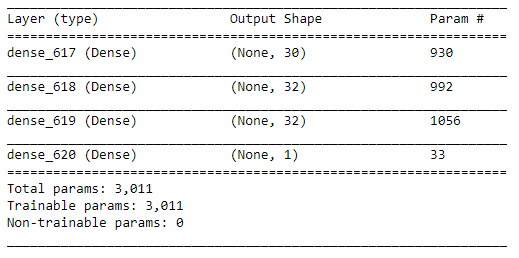
\includegraphics[width=.7\textwidth]{images/archshitty.PNG}
  \caption{Sample Architecture of Credit Card ANN}
  {Note: Simply remove one of the hidden 32 node dense layer to get the other network's configuration.}
\end{figure}

\begin{figure}
  \centering
  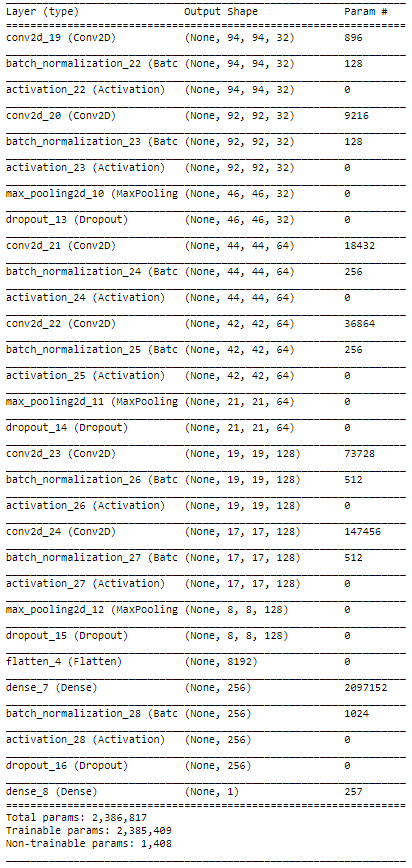
\includegraphics[width=.6\textwidth]{images/arch.PNG}
  \caption{Sample Architecture of PCam CNN with BatchNorm before ReLU.}
  {Note: Simply swap the activation and batch-norm to get the other network's configuration.}
\end{figure}

\subsection{Credit Card Fraud}
For credit card fraud, we're back to k=10 for cross validation -- cross-validating the under-sampled dataset is not too taxing. Each fold of k-fold took a little less than a minute on average; training and cross validating all 8 models took 55 minutes.
\subsubsection{Finding Hyper-parameters}
Only batch-size=32 and number of dense nodes per hidden layer (32) were held constant for this dataset. A detailed view of the single layer model can be seen in figure 4. I cross-validated 8 different models with the following hyper-parameter sets: $learningRate = \{.001,  .0005\}$, $layers = \{1,  2\}$, and $l1 = \{.1,  .01\}$. Surprsingly all 8 models performed equally well (94.9\%), when early stopped at different epochs, with a max accuracy difference of +- .001\% (see figure 6 for a loss and accuracy graphs of the top 3 of these models). The rest of the models also performed relatively well too, with the lowest accuracy being 91\%. 

For the simplest model [learningRate = 0.001, l1 = .1, layers = 1], the early stopping needed to occur earlier at 25 epochs (compared to 75 and 50), possibly due to the lower regularization rate. Because of Occam's Razor, I decided to use this model @ 25 epochs for final testing in my comparative analysis.
\begin{figure}
  \centering
  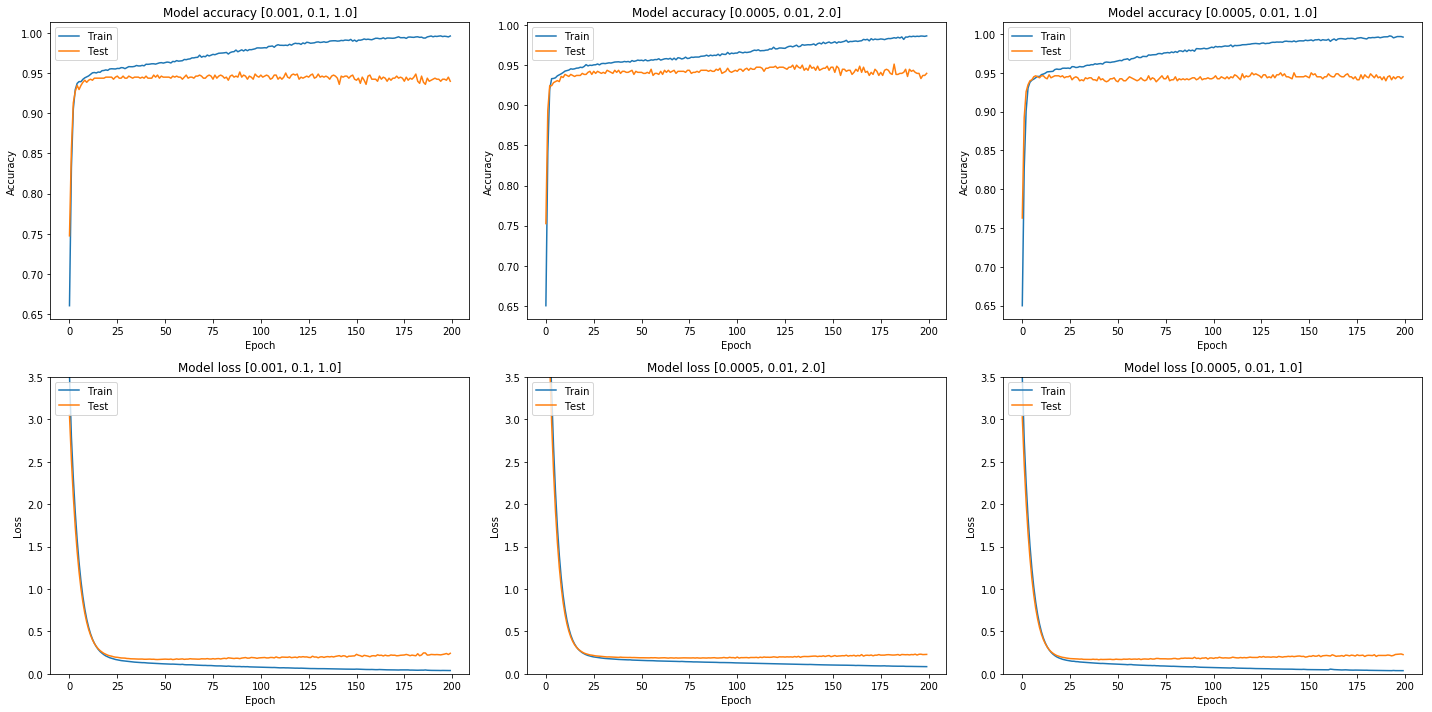
\includegraphics[width=1\textwidth]{images/best_nns.png}
  \caption{Mean 10-fold Loss/Accuracy graphs of Fraud ANNs; increasing to decreasing performance (left to right).}
  {Note: The title follows this format: [learning rate, l1, and layers], and the loss function is binary cross-entropy.}
\end{figure}
\section{K-NN}
\textcolor{red}{For K-NN, I decided to switch to Random Hyper-parameter search. This choice will be revisited in the comparative analysis section.}
For this subsection, let k in cross fold validation be 10; also, weights for kNN were set to uniform. 
\subsection{PCam}
\subsection{Note on Feature Engineering}
For K-NNs, my models took a prohibitively long amount of time to query and test on a dataset. Each fold of 10-fold on the raw image itself took 10 hours; after the first fold, I stopped the training process. I downsampled the image to 8x8, converted it to black and white, AND used PCA (fit on the entire training set). For PCA decompositon, I set the num\_components value to .4. At this level of compression, I'd be happy with a trivial classifier. 

The good news is that each fold took 10 minutes to complete (where all of the computation time fit into the testing portion of k-fold, due to K-NNs lazy learning methods). All in all, the entire process took 8.54 hours.
\subsubsection{Finding Hyper-parameters}
For this dataset, the following sets define our hyper-parameter search space:  $powerParameter = \{\| x\|, {\| x\|}_{2}\}$ and $numNearestNeighboors = \{rand(1...100)\}$. Sci-kit learn's $randomSearchCV$ was set to use 5 iterations of randomSearch.

Random guessing has an accuracy rate of 50\%, but our best estimator (neighboors=48, powerParam=${\| x\|}_{2}$) had a "whopping" accuracy rate of 57.8\%. There does appear to be a log-relationship between neighboors and accuracy, but there aren't enough datapoints to make a concrete conclusion (see Fig. 7).
\subsection{Credit Card Fraud}
\subsubsection{Finding Hyper-parameters}
For this dataset, the following sets define our hyper-parameter search space:  $powerParameter = \{\| x\|, {\| x\|}_{2}\}$ and $numNearestNeighboors = \{rand(2...20)\}$. Weights for kNN were set to uniform, and Sci-kit learn's $randomSearchCV$ was set to use 50 iterations of randomSearch. 

Our best estimator (neighboors=3, powerParam=${\| x\|}_{2}$) had a mean k-fold accuracy of 94.8\%. The distribution of other parameters can be seen in figure 7; all perform above the 90\% range, yet there doesn't appear to be a discernable pattern in hyperparameter choice and model performance

\begin{figure}
  \centering
  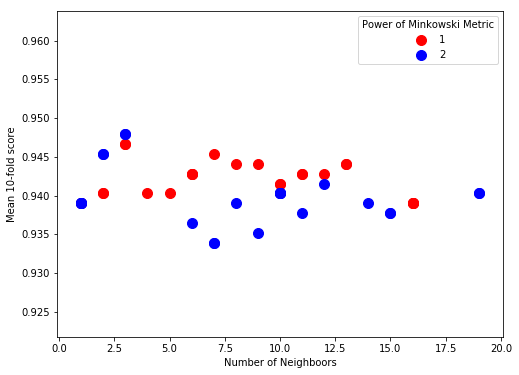
\includegraphics[width=.45\textwidth]{images/kNN_Credit.png}
  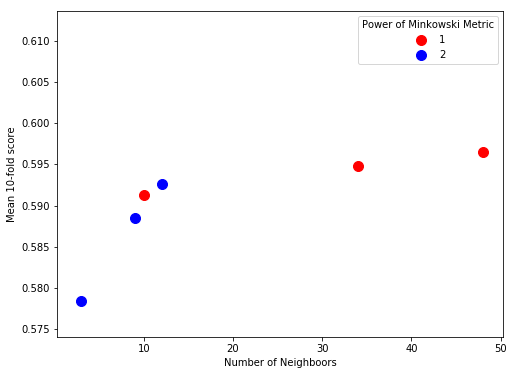
\includegraphics[width=.45\textwidth]{images/kNN_pcam.png}
  \caption{Mean 10-fold accuracy of Credit Card (left) and PCam (right) models.}
\end{figure}
\section{Boosting}
For this section, I used decision trees from the ones I experimented with in the earlier section, and boosted them with AdaBoost. Note that I will not use a very complex model if another simpler one exists with reasonable accuracy. With the credit card dataset, I hit 93.15\% accuracy with $leafLimit= 76$ and $depth= 5$ -- more complex models were not better. However, for PCam, complex models were marginally better. The PCam boosted decision tree in the next subsection did not use $leafLimit = depthLimit = 200$ with 71\% cross-validation accuracy; instead, it used $leafLimit= 76$ and $depth= 200$ with a 70.5\% accuracy.

My reasoning behind this is that the weak learners themselves should not be too complex, in order to avoid overfitting\autocite{Udacity-Adaboost}. Also, assume k=10 for cross validation in this section. 
\subsection{Exploring Hyperparameter Choices}
I found the following, very interesting quote on StackExchange citing literature that highlights the training behaviour of adaptive boosted models.
\begin{quote}
Mease and Wyner argue that AdaBoost should be run for a long time, until it converges, and that 1,000 iterations should be enough \autocite{mease2008evidence}. The main point of the paper is that the intuition gained from the "Statistical view of boosting" due to Friedman, Hastie, and Tibshirani could be incorrect, and that this applies to their recommendations to regularize AdaBoost with early stopping times \autocite{hastie01statisticallearning}. Their results suggest that long running times, no regularization, and deep trees as base learners make use of AdaBoost's strengths.

Friedman, Hastie, and Tibshirani respond to Mease and Wyner with a demonstration that AdaBoost with decision stumps, shrinkage, and early stopping can perform better than deep trees, no shrinkage and running until convergence, but their argument depended on running the algorithm to convergence anyway \autocite{hastie01statisticallearning}. That is, even if 100 or 10 iterations are optimal, it is necessary to run many hundred iterations to find out where the correct stopping point should be.\autocite{Stackoverflow-quote}
\end{quote}
Using these intuitions, I would pick hyperparameters to train Adaboost.
\subsection{PCam}
\subsubsection{Finding Hyper-parameters}
For PCam, I tried two different values for hyperparameters: numEstimators = 10 and numEstimators = 100. Because of the long cross-validation times, I would not test more parameters if it appeared that Adaboost converged.

\begin{center}
\begin{tabular}{ |c|c|c|c| } 
\hline
Number of Estimators & \begin{math}\mu\end{math} 10-fold score & Training Time \\
\hline
Baseline & .705 & 10 minutes \\ 
10 & .696 & 1.2 Hours\\ 
100 & .689 & 11.7 Hours\\ 

\hline
\end{tabular}
\end{center}
Because of the small difference in 10-fold scores, I assumed that Adaboost did in fact converge. I could not test higher values for estimators because of computational limits. For final testing, I will use less estimators because of Occams Razor, because empirical performance of n=10 was higher, and because of the aforementioned intuitions. Adaboost, oddly, did \textbf{\textit{worse}} than the baseline decision tree. This will be explored in comparative analysis.
\subsection{Credit Card Fraud}
\subsubsection{Finding Hyper-parameters}
The following set defines our hyper-parameter search space: $numEstimators = \{rand(1...1000)\}$. I picked 50 choices from numEstimators, and included the 51st example to be numEstimators=1000 just to follow the aforementioned intuitions. The best accuracy rate acheived was 94.8\% with numEstimators=17. It appears that Adaboost converges after the 50 estimator mark -- soon therafter, the accuracy fluctuates between 94\% and 95\%. Figure 8 shows the hyperparameter search space.
\begin{figure}
  \centering
  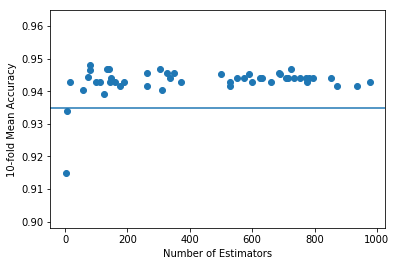
\includegraphics[width=.6\textwidth]{images/boosting_acc.png}
  \caption{Mean 10-fold Loss/Accuracy on Credit Card Fraud for various choices of iterations/estimators in AdaBoost.}
  {Note that the horizontal line is the baseline, unboosted, decision tree.}
\end{figure}
\section{Support Vector Machines}
All SVMs tested in the following subsection were C-support SVMS. Assume k = 3 for SVMs, and k = 10 for Credit Card Fraud.
\subsection{PCam}
\subsubsection{Note on Feature Engineering}
I follow the same PCA decomposition in Boosting, except that num\_components = .7
\subsubsection{Finding Hyper-parameters}
For this dataset, the following sets define our hyper-parameter search space:  $kernel = \{linear, rbf\}$ and $penalty = \{50, 100\}$. Because of time constraints, I used a grid search for only those parameters. Our best estimator (C=100, kernel=rbf) had a mean 10-fold accuracy of 54.9\%. The following table\footnote{The training times were not recorded for SVM PCam Training -- the table consists of rough estimates.} shows the hyperparameter seach space. 
\begin{center}
\begin{tabular}{ |c|c|c|c| } 
\hline
Kernel & Penalty & \begin{math}\mu\end{math} 10-fold score & Training Time\\
\hline
Linear & 50 & .521 & 24 Hours\\ 
rbf & 50 & .474 & 24 Hours\\ 
Linear & 100 & .549 & 24 Hours\\ 
rbf & 100 & .488 & 24 Hours\\ 
\hline
\end{tabular}
\end{center}

\subsection{Credit Card Fraud}
\subsubsection{Finding Hyper-parameters}
For this dataset, the following sets define our hyper-parameter search space:  $kernel = \{linear, rbf, sigmoid\}$ and $penalty = \{rand(1...300)\}$. Sci-kit learn's $randomSearchCV$ was set to use 666 iterations of randomSearch. Our best estimator (C=199, kernel=linear) had a mean 10-fold accuracy of 94.16\%. Because of the linear kernel's superior performance, I suspect that my data may be close to linearly separable. Figure 9 shows the hyperparameter search space.
\begin{figure}
  \centering
  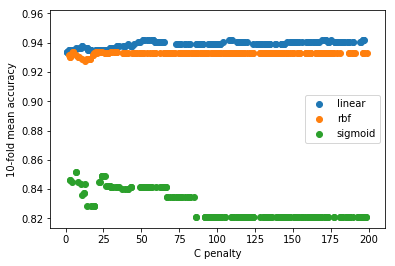
\includegraphics[width=.6\textwidth]{images/svm.png}
  \caption{Mean 10-fold Accuracy on Credit Card Fraud for various choices of kernels/penalties in SVM.}
\end{figure}
\section{Comparative Analysis}
\subsection{Chosen Parameters \& Accuracy}
The following tables summarize our best parameters and their CV accuracy during training.
\begin{center}
Hyperparameter \& CV Accuracy Tables
\begin{tabular}{ |c|c|c|c| } 
\hline
Model Type & PCam Parameters & Fraud Parameters \\
\hline
Decision Tree & leafLimit = depthLimit = 200 & leafLimit = 76, depthLimit = 5\\ 
Neural Networks & learningRate = .001, see Fig. 5 & learningRate = .001, layers = 2, lr = 1, see Fig. 4\\ 
k Nearest Neighbors & neighbors = 48, powerParam = 2 & neighbors = 3, powerParam = 2\\ 
Boosted Decision Tree & numEstimators = 10 & numEstimators = 17\\ 
SVM & kernel = rbf, C = 100 & kernel = linear, C = 199\\ 
\hline
\end{tabular}
\end{center}

\begin{center}
\begin{tabular}{ |c|c|c|c| } 
\hline
Model Type & PCam CV Accuracy & Fraud CV Accuracy \\
\hline
Decision Tree & .710 & .932 \\ 
Neural Networks & .889 & .949 \\ 
k Nearest Neighbors & .578 & .948 \\ 
Boosted Decision Tree & .689 & .948 \\ 
SVM & .549 & .942 \\ 
\hline
\end{tabular}
\end{center}
\subsection{Learning Curves on the Withheld Testing Datasets}
\subsubsection{PCam}
Essentially, the only algorithims that appeared to learn (at all) were decision trees and the neural network (see Fig 10). Because of batch gradient descent, the neural network found an minima very quickly, so the learning curve itself isn't very clear (you cannot see it move from .5 to .9, because on the first tenth of the dataset, it has started converging rapidly). Boosting and Decision Trees follow the same learning curve; my hypothesis is that the base estimator for the Boosted Decision tree is still too complex, so the learning isn't that different from a regular decision tree. Future steps could include using an even simpler estimator.

Finally, SVM and kNN perform the worst. There is no learning at all. They border around chance, possibly because of my very liberal feature engineering.
\begin{figure}
  \centering
  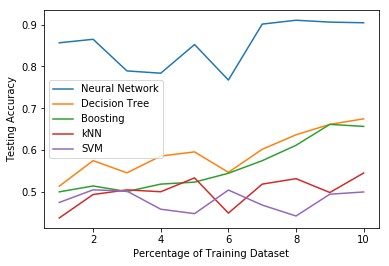
\includegraphics[width=.5\textwidth]{images/pcam_tests.png}
  \caption{Accuracy Learning Curves for PCam.}
\end{figure}
\subsubsection{Credit Card Fraud}
Looking at the training/testing graphs for every learning algorithm subsection, I think I've established that it is pretty easy to classify the undersampled subset of credit card fraud data; however, classification accuracy is very different from precision and recall. On an oversampled dataset, getting most of the data correctly classified is trivial -- however, our ability to classify each category correctly is far more important. For example, note our Neural Network algorithm subsection: each variant neural network had similar, very high, accuracy rates on k-fold validation. This subsection, however, will emphasize precision and recall -- not just accuracy.

To do this, we'll use the AUC-ROC metric: essentially, it just takes the area under a precision-recall graph. We'll test both our withheld 20\% of our undersampled dataset, and the final, entire dataset. I'm expecting high accuracy scores for the withheld 20\%, since our k-fold all around was pretty high (above 90\% for the best estimator from each algorithm). Figure 11 highlights the final learning curves for the Credit Card Fraud dataset, on both testing datasets.

Note that the entire dataset curve does not follow a typical learning curve pattern. Instead, it's more akin to trial by fire. Each added percent chunk of the entire testing dataset challenges our classifier's ability to generalize, since our classifier was relatively easy to train. Both boosted decision trees and decision trees fail at the same point, which suggests that a key branch in the decision tree fails to generalize for the withheld dataset. This isn't seen in the remaining models. Interpreting the each percentage chunk as another trail also highlights which points in the dataset cause this failure in generalization.

The model that learns the "best," with respect to the learning curve, is k Nearest Neighbors. By best, I mean isn't fooled by each new percentage of train/test data. Surprisingly, it follows a steadily increasing pattern; although I expected the ROC-AUC score to fall every-time new chunks of the entire dataset is provided, it climbs. Plus, being a lazy learner (compared to the rest of the models), it would be well suited to active learning. The ANN, although having better final performance, is very erratic in comparison. 
\begin{figure}
  \centering
  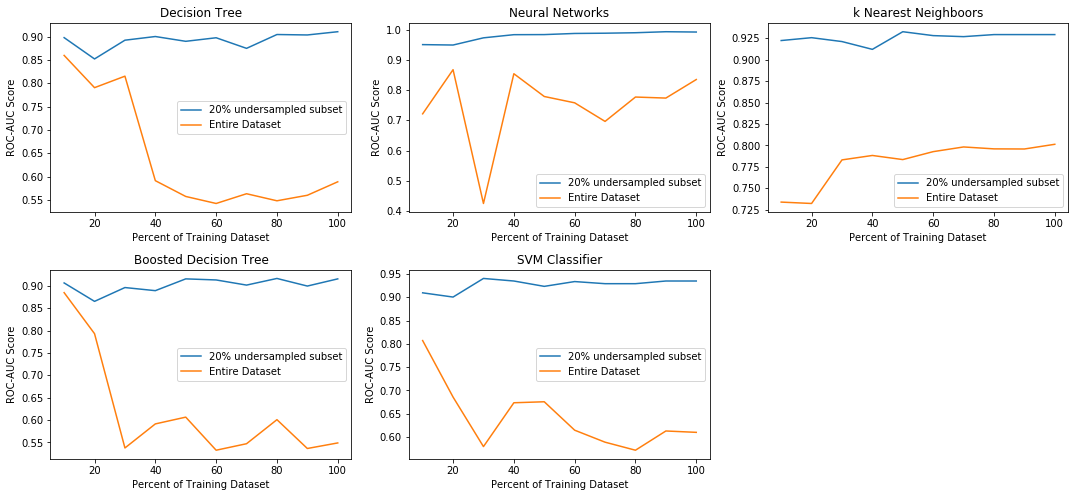
\includegraphics[width=1\textwidth]{images/trialbyfire.png}
  \caption{ROC-AUC Learning Curves for Credit Card Fraud.}
\end{figure}
\subsection{Accuracy and Speed Tradeoffs}
The following tables categorize speed of models across training/CV and testing (on the final dataset). Before reading the tables, note that I used a different number of iterations for random search based on how big my search space was. I varied my search spaces between algorithms; therefore, the hyperparater search times aren't necessarily a metric of how fast the algorithm itself is. Instead, it's how long it takes for me to find a good set of hyperparameters.

The testing/fitting time would more accurately represent performance.
\subsubsection{PCam}
\begin{center}
\begin{tabular}{ |c|c|c|c| } 
\hline
Model Type & Withheld Testing Accuracy & Hyperparameter Search \& CV Time & Testing/Fitting Time \\
\hline
Decision Tree & .674 & 16.4 hours & 1.1 hours\\ 
Neural Networks & .904 & 3.33 hours & 45 mins\\ 
k Nearest Neighbors & .544 & 8.54 hours & 2.2 hours\\ 
Boosted Decision Tree & .656 & 12.9 hours & 3.5 hours\\ 
SVM & .499 & Roughly 4 days? Not fun. & 10.3 hours\\ 
\hline
\end{tabular}
\end{center}
I guess I now know why CNNs are a good idea for image classification.
Every algorithim does horribly (a little better than random chance) except for the decision tree -- only that with the decision tree, I had time to do nearly an exhaustive search of the hyperparameter space. With the other models, that was impossible due to time constraints. To get kNN and SVM to even run required serious compression with PCA, to a point where the original data was unrecognizable. Even then, sci-kits implementation of these algorithms took up 28 GB of RAM on average, compared to the maximum 16 GB RAM + 8 GB VRAM usage for Keras' CNN. For Keras, the images were also uncompressed, unlike the rest of the ML algorithms.

Just use a CNN. With less epochs (only 5!) the model annihilates its competition.
\subsubsection{Credit Card Fraud}
\begin{center}
\begin{tabular}{ |c|c|c|c| } 
\hline
Model Type & Entire Dataset AUC Score & Hyperparameter Search \& CV Time & Testing/Fitting Time \\
\hline
Decision Tree & .589 & 3.2 mins & .029 sec\\ 
Neural Networks & .835 & 55 mins & 4.63 sec\\ 
k Nearest Neighbors & .801 & 2.7 sec & 1.86 sec\\ 
Boosted Decision Tree & .549 & 8.6 mins & .044 sec\\ 
SVM & .601 & 50.59 secs & 3.00 sec\\ 
\hline
\end{tabular}
\end{center}
Based on the above table, I would fail to consider the base decision tree or its boosted counterpart. Neither perform well when tested on the final testing dataset. The two competitors here are kNN and the simple ANN. The neural network performs very well on the final dataset; however, training and testing times are significantly higher than kNNs. Also, when putting a model into production, kNNs do not have to be repeatedly retrained, thanks to their lazy learning attributes.

If I'm required to score high with lots of compute power, while avoiding misclassification on a streaming dataset of credit card transactions, the high compute would make ANNs feasible. Otherwise, I'd stick through with kNN. 

\subsection{Extended Q\&A/Final Thoughts}
\subsubsection{Why exactly does the CNN perform so much better for image classification, accuracy and performance wise? Do you regret picking an image dataset?}
I am very very angry (jk <3 you TAs) that I had to waste my time on SVMs and kNNs. Both of these algorithims took forever, whereas the CNN converged rapidly. Turns out, this all ties into a core similarity between SVMs and kNNs. Stanford's CS 231n course on computer vision comes to the following conclusion: 
\begin{quote}
The use distance metrics on raw pixel values is not adequate since the distances correlate more strongly with backgrounds and color distributions of images than with their semantic content.\autocite{Stanford-Img} 
\end{quote}
SVMs and kNNs use distance metrics to pick margins, which puts them at a severe disadvantage compared to CNNs. The SVM took especially long because, according to sci-kit's documentation, the fit run-time has a big O that's more than quadratic due to the underlying quadratic programming problem it needs to solve. I also suspect that added GPU power and less training epochs helped the CNN.

Nope, don't regret the image dataset. Learned a lot through the pain, but I'll use Google Cloud compute next time lol.
\subsubsection{Why should I avoid Grid-Search?}
This fantastic paper (Bergstra, Bengio) puts it pretty well:
\begin{quote}
Compared with neural networks configured by a pure grid search, we find that random search over the same domain is able to find models that are as good or better within a small fraction of the computation time. Granting random search the same computational budget, random search finds better models by effectively searching a larger, less promising configuration space.\autocite{bergstra2012random}
\end{quote}
\subsubsection{Why did Adaboost do \textbf{\textit{worse}} then the regular decision tree with PCam?}
I wasn't able to do a thorough search of the hyper-parameter space, but I still suspect that my underlying model was too complex, even though I tried to take measures to ensure it was not. Because of this, boosted decision tree accuracy would fluctuate around the regular decision tree (and in my case lower than), based on the number of estimators.
\subsubsection{Why did you use PCA instead of auto-encoders?}
I didn't know what auto-encoders were until I wrote this section, but I'll make up an excuse: I didn't want to introduce non-linearities in my feature engineering.
\subsubsection{Why did you pick larger batch-sizes for the Neural Networks?}
Very large batch-sizes (batchsize > 512) result in the model's inability to generalize\autocite{DBLP:journals/corr/KeskarMNST16}. 

\printbibliography

\end{document}